%
% File acl2015.tex
%
% Contact: car@ir.hit.edu.cn, gdzhou@suda.edu.cn
%%
%% Based on the style files for ACL-2014, which were, in turn,
%% Based on the style files for ACL-2013, which were, in turn,
%% Based on the style files for ACL-2012, which were, in turn,
%% based on the style files for ACL-2011, which were, in turn, 
%% based on the style files for ACL-2010, which were, in turn, 
%% based on the style files for ACL-IJCNLP-2009, which were, in turn,
%% based on the style files for EACL-2009 and IJCNLP-2008...

%% Based on the style files for EACL 2006 by 
%%e.agirre@ehu.es or Sergi.Balari@uab.es
%% and that of ACL 08 by Joakim Nivre and Noah Smith

\documentclass[11pt]{article}
\usepackage{acl2015}
\usepackage{times}
\usepackage{url}
\usepackage{latexsym}
\usepackage{amsopn}

%%%%%%%%%%%%%%%%%%%%%%%%%%%%%%%%%%%%%%%%%%%%%%%%%%%%%%%%%%%%%%%%%%%%
%% KUI'S STANDARD PREAMBLE
%%%%%%%%%%%%%%%%%%%%%%%%%%%%%%%%%%%%%%%%%%%%%%%%%%%%%%%%%%%%%%%%%%%%

\usepackage{subfigure}
\usepackage{algorithm}
\usepackage{algorithmicx}
\usepackage{algpseudocode}
\usepackage{xcolor}
\usepackage{tabularx}

\usepackage{graphicx}
\DeclareMathOperator{\conv}{conv}
\DeclareMathOperator{\st}{s.t.}
\DeclareMathOperator{\dom}{dom}
\DeclareMathOperator{\im}{im}
\DeclareMathOperator{\Ne}{Ne}
\DeclareMathOperator{\sign}{sign}
\DeclareMathOperator{\Var}{Var}
\DeclareMathOperator{\diag}{diag}
\DeclareMathOperator{\vvec}{vec}


%\setlength\titlebox{5cm}

% You can expand the titlebox if you need extra space
% to show all the authors. Please do not make the titlebox
% smaller than 5cm (the original size); we will check this
% in the camera-ready version and ask you to change it back.

\title{Topic Models for Texts and Images in Representation Space}

\author{Kui Tang \\
  Columbia University \\
  {\tt kt2384@columbia.edu} \\\And
  Sameer Lal \\
  Columbia University \\
  {\tt sl3368@columbia.edu} \\}
%\date{10 May 2015}
\date{}

\begin{document}
\maketitle
\begin{abstract}
The abstract goes here.
\end{abstract}

\section{Introduction}

\section{Related Work}
\paragraph{Neural multimodal models.}
\cite{Lecun98} propose joining several neural network models for multimodal learning into a joint objective function, and then optimizing the parameters of each to maximize performance on this joint measure. \cite{Srivastava14} propose a joint text-image model using RBMs. Their model is fully generative, and the textual model is an undirected analogue to a topic model. However, they are unable to leverage state-of-the-art CNN image features, and they rely on contrastive divergence for learning, which limits scalability. They also rely on a binary semantic space, while ours is real.

\paragraph{Topic models on shallow image features.}
Several authors have applied topic modeling to visual or joint text and visual data, but none to date have utilized deep semantic representations as image features. \cite{Barnard03} considers several models beginning with marginally independent emission distributions for words and image blobs (which are nevertheless conditional dependent) and proceeds to model additional dependencies between the distributions. \cite{Wang09} model alignment between words and image patches, but train on a supervised dataset and use only bag of codeword features to represent images, with codewords generated by $k$-means and SIFT. Moreover, these methods are designed only for supervised image captioning.

Some work has used topic models in unsupervised settings for images. \cite{Fritz08} trains LDA to detect object categories, but they use only gradient histogram representations. \cite{Cao07} proposed a model for unsupervised object detection, but they only used quantized SIFT features.

\paragraph{Hybrid neural network and HMM models.}
A simpler problem related to our work is to combine output from a feedforward neural network with a Hidden Markov model. Several authors have proposed schemes tuned for a variety of tasks \cite{Trentin01}. The approach closest to ours is that of \cite{Bengio92}, which derives gradient updates to a feedforward neural network based on the maximum-likelihood objective. Our work shares the same approach to optimize the neural network parameters to maximize the likelihood of the overall probabilistic model.

\section{Model}

\section{Results}
\begin{figure}
\centering
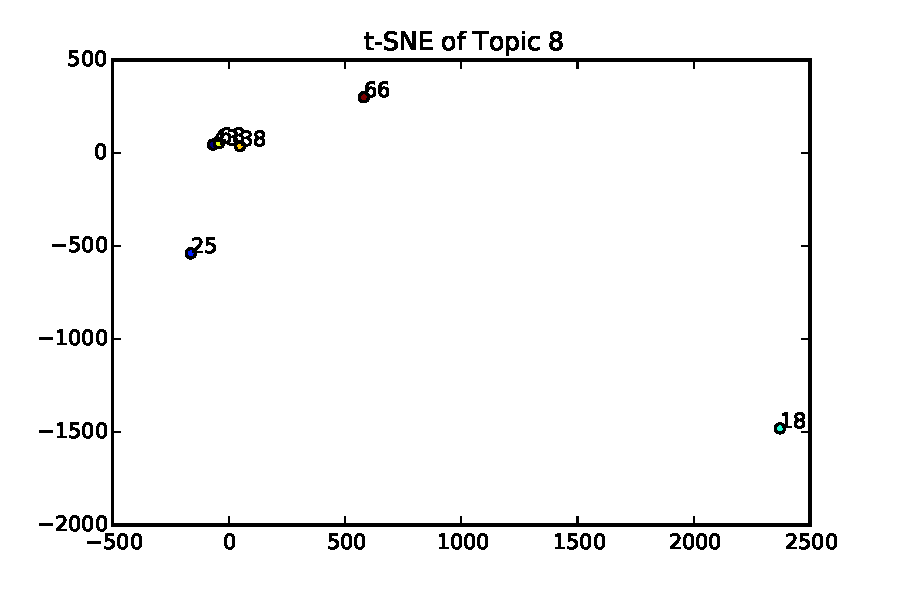
\includegraphics[width=0.5\textwidth]{assets/gtm100_topic8_tsne.pdf}
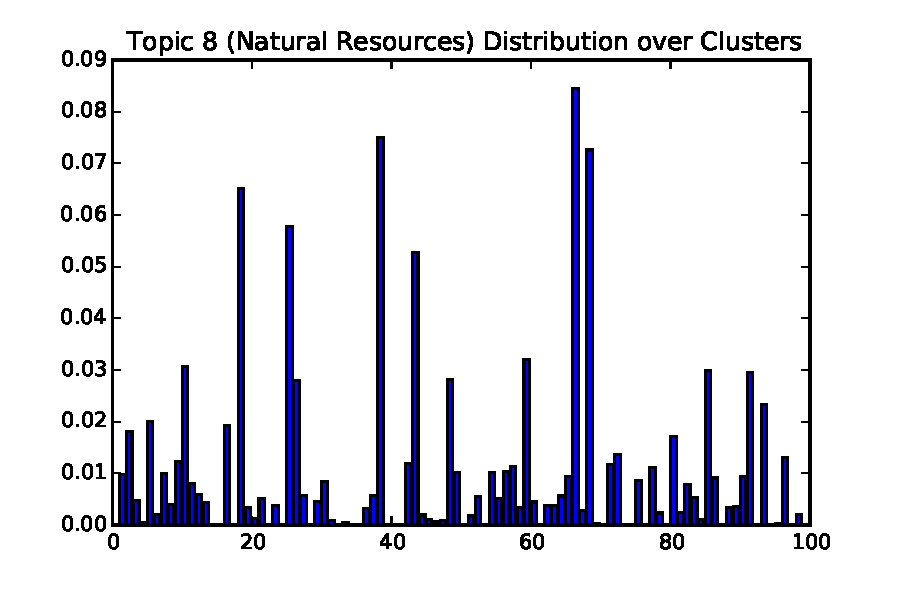
\includegraphics[width=0.5\textwidth]{assets/gtm100_topic8_probs.pdf}
\caption{\emph{Top:} Locations of means of significant ($\geq 5\%$ posterior probability) clusters for the ``natural resources'' topic. \emph{Bottom:} Distribution over clusters for the ``Natural resources'' topic.}
\end{figure}

\section{Discussion}

\subsection{Footnotes}

{\bf Footnotes}: Put footnotes at the bottom of the page and use 9
points text. They may be numbered or referred to by asterisks or other
symbols.\footnote{This is how a footnote should appear.} Footnotes
should be separated from the text by a line.\footnote{Note the line
separating the footnotes from the text.}

\subsection{Graphics}

{\bf Illustrations}: Place figures, tables, and photographs in the
paper near where they are first discussed, rather than at the end, if
possible.  Wide illustrations may run across both columns.  Color
illustrations are discouraged, unless you have verified that  
they will be understandable when printed in black ink.

{\bf Captions}: Provide a caption for every illustration; number each one
sequentially in the form:  ``Figure 1. Caption of the Figure.'' ``Table 1.
Caption of the Table.''  Type the captions of the figures and 
tables below the body, using 11 point text.


\section{XML conversion and supported \LaTeX\ packages}

Following ACL 2014 we will also we will attempt to automatically convert 
your \LaTeX\ source files to publish papers in machine-readable 
XML with semantic markup in the ACL Anthology, in addition to the 
traditional PDF format.  This will allow us to create, over the next 
few years, a growing corpus of scientific text for our own future research, 
and picks up on recent initiatives on converting ACL papers from earlier 
years to XML. 

We encourage you to submit a ZIP file of your \LaTeX\ sources along
with the camera-ready version of your paper. We will then convert them
to XML automatically, using the LaTeXML tool
(\url{http://dlmf.nist.gov/LaTeXML}). LaTeXML has \emph{bindings} for
a number of \LaTeX\ packages, including the ACL 2015 stylefile. These
bindings allow LaTeXML to render the commands from these packages
correctly in XML. For best results, we encourage you to use the
packages that are officially supported by LaTeXML, listed at
\url{http://dlmf.nist.gov/LaTeXML/manual/included.bindings}

\section*{Acknowledgments}

We thank Profs. Liangliang Cao and James Fan for organizing a deep learning course, encouraging us to explore multimodal models, and for their advice on evaluation.

% include your own bib file like this:
\bibliographystyle{acl}
\bibliography{ML}

%\begin{thebibliography}{}
%\end{thebibliography}

\end{document}
